\documentclass[14pt]{standalone}
\usepackage{tikz}
\usepackage{pgfplots}
\usetikzlibrary{positioning}
\usetikzlibrary{arrows}


\begin{document}
  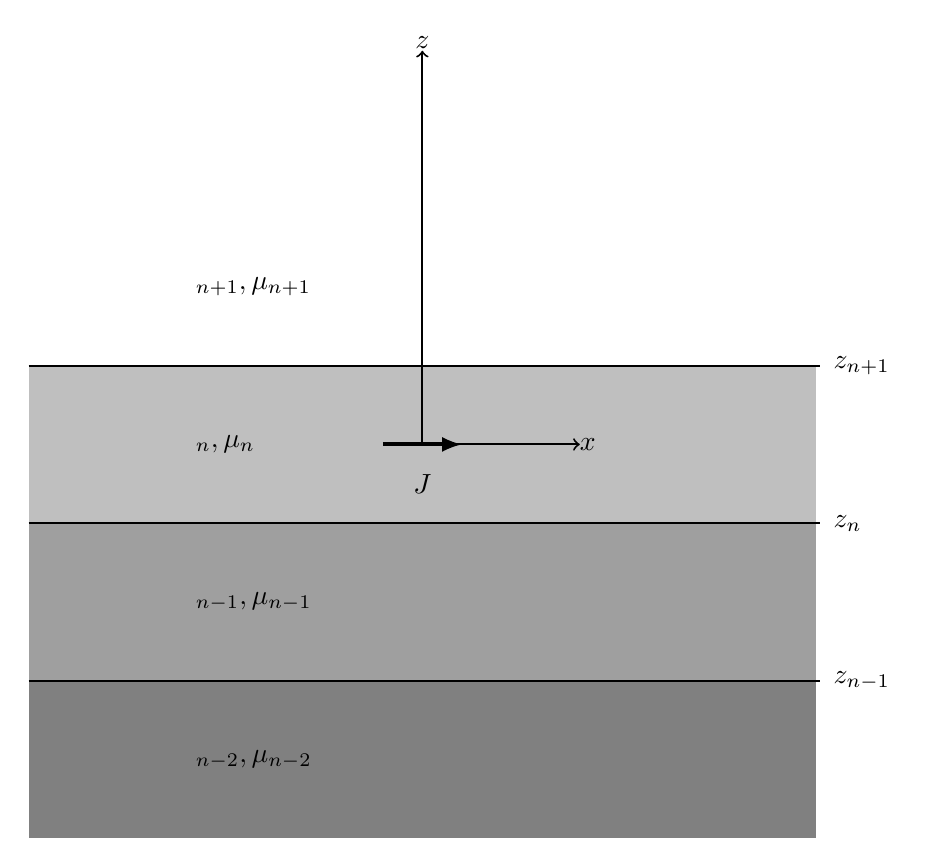
\begin{tikzpicture}
    % Draw Layers
    \fill [fill = gray] (0.0,-3.0) rectangle (10,-1);
    \fill [fill = gray!75] (0.0,-1.0) rectangle (10,1);
    \fill [fill = gray!50] (0.0,1) rectangle (10,3);
    \fill [fill = white] (0.0,3) rectangle (10,5); % Draw without border

    %% Draw coordinate system
    % x-axis
    \draw [line width=0.25mm,->] (5, 2) -- (7, 2);
    % z-axis
    \draw [line width=0.25mm,->] (5, 2) -- (5, 7);
    % Unit x-axis label
    \node at (7.1, 2) {$x$};
    % Unit z-axis label
    \node at (5, 7.1) {$z$};

    %% Source and label (use arrows command to insert arrow of choice)
    \draw [line width = 0.5mm,arrows={-latex}] (4.5, 2) -- (5.5, 2);
    \node at (5, 1.5) {$J$};

    %% Dimensioning
    % Lowest
    \draw [line width=0.25mm] (0, -1) -- (10.05, -1);
    \node [anchor=west] at (10.1, -1) {$z_{n-1}$};
    % Lower
    \draw [line width=0.25mm] (0, 1) -- (10.05, 1);
    \node [anchor=west] at (10.1, 1) {$z_{n}$};

    %Upper
    \draw [line width=0.25mm] (0, 3) -- (10.05, 3);
    \node [anchor=west] at (10.1, 3) {$z_{n+1}$};

    %% Labeling
    % Lowest
    \node [anchor=west] at (2, -2) {$\E_{n-2}, \mu_{n-2}$};

    % Lower
    \node [anchor=west] at (2, 0) {$\E_{n-1}, \mu_{n-1}$};

    % Middle
    \node [anchor=west] at (2, 2) {$\E_{n}, \mu_{n}$};

    % Upper
    \node [anchor=west] at (2, 4) {$\E_{n+1}, \mu_{n+1}$};

  \end{tikzpicture}
\end{document}
